\chapter{Interfacce e Classi Astratte}
\label{cap:interfacce_classi_astratte}

\section*{Obiettivi di apprendimento}
Al termine di questo capitolo sarai in grado di:
\begin{itemize}
    \item Comprendere il concetto di astrazione nella programmazione orientata agli oggetti
    \item Dichiarare e implementare interfacce Java
    \item Creare e utilizzare classi astratte
    \item Distinguere quando usare interfacce o classi astratte
    \item Applicare il polimorfismo attraverso interfacce e classi astratte
\end{itemize}

\section{Il concetto di astrazione}

L'\textbf{astrazione} è uno dei quattro principi fondamentali della programmazione orientata agli oggetti (insieme a incapsulamento, ereditarietà e polimorfismo). Consiste nel definire \textit{cosa} fa un oggetto (le sue responsabilità e il suo comportamento pubblico) senza specificare \textit{come} lo fa (i dettagli implementativi). In Java, l'astrazione si realizza principalmente attraverso interfacce e classi astratte.

L'astrazione permette di:
\begin{itemize}
    \item Definire contratti (insiemi di metodi) che le classi devono rispettare
    \item Separare la specifica del comportamento dalla sua implementazione concreta
    \item Scrivere codice più flessibile, manutenibile e testabile
    \item Facilitare il lavoro in team (ogni sviluppatore implementa le proprie classi rispettando il contratto comune)
    \item Nascondere la complessità implementativa, esponendo solo le operazioni essenziali
\end{itemize}

\section{Interfacce}

Un'\textbf{interfaccia} in Java è un tipo di riferimento che definisce un insieme di metodi astratti (senza implementazione) che le classi devono implementare. È un contratto: se una classe dichiara di implementare un'interfaccia, si impegna a fornire il codice per tutti i metodi dichiarati.

\subsection{Dichiarazione di un'interfaccia}

\begin{lstlisting}
public interface Forma {
    // Metodi astratti (implicitamente public abstract)
    double calcolaArea();
    double calcolaPerimetro();

    // Costanti (implicitamente public static final)
    double PI = 3.14159;
}
\end{lstlisting}

Questo esempio mostra la struttura base di un'interfaccia in Java. L'interfaccia \texttt{Forma} definisce un \textbf{contratto} che tutte le classi che la implementano devono rispettare. In particolare, dichiara due metodi astratti: il metodo \texttt{oggetto.calcolaArea()} e il metodo \texttt{oggetto.calcolaPerimetro()}, che non hanno implementazione nell'interfaccia stessa. Ogni classe che implementerà \texttt{Forma} dovrà fornire il codice concreto per questi metodi. Inoltre, l'interfaccia definisce una costante \texttt{Forma.PI}, che è automaticamente \texttt{public}, \texttt{static} e \texttt{final}. Questo significa che il valore della costante \texttt{Forma.PI} può essere utilizzato da qualsiasi classe senza istanziare l'interfaccia e non può essere modificato. Le interfacce sono utili per definire comportamenti comuni che possono essere condivisi da classi completamente diverse senza imporre una relazione gerarchica tra di esse.

\begin{nota}
In un'interfaccia:
\begin{itemize}
    \item I metodi dichiarati sono implicitamente \texttt{public} e \texttt{abstract}
    \item Le variabili dichiarate sono implicitamente \texttt{public}, \texttt{static} e \texttt{final} (costanti di classe)
    \item Non si possono dichiarare variabili di istanza (attributi non statici)
\end{itemize}
\end{nota}

\subsection{Implementare un'interfaccia}

Una classe implementa un'interfaccia usando la parola chiave \texttt{implements} e deve fornire l'implementazione di tutti i metodi dichiarati nell'interfaccia.

\subsection{Esempio 1: Interfaccia Forma con implementazioni}

\begin{lstlisting}
// Interfaccia
public interface Forma {
    // Metodi astratti dell'interfaccia
    double calcolaArea();
    double calcolaPerimetro();
}

// Implementazione: Rettangolo
public class Rettangolo implements Forma {
    // Attributi di istanza
    private double base;
    private double altezza;

    // Costruttore
    public Rettangolo(double base, double altezza) {
        this.base = base;
        this.altezza = altezza;
    }

    // Implementazione del metodo rettangolo.calcolaArea()
    @Override
    public double calcolaArea() {
        return base * altezza;
    }

    // Implementazione del metodo rettangolo.calcolaPerimetro()
    @Override
    public double calcolaPerimetro() {
        return 2 * (base + altezza);
    }
}

// Implementazione: Cerchio
public class Cerchio implements Forma {
    // Attributi di istanza e costanti
    private double raggio;
    private static final double PI = 3.14159;

    // Costruttore
    public Cerchio(double raggio) {
        this.raggio = raggio;
    }

    // Implementazione del metodo cerchio.calcolaArea()
    @Override
    public double calcolaArea() {
        return PI * raggio * raggio;
    }

    // Implementazione del metodo cerchio.calcolaPerimetro()
    @Override
    public double calcolaPerimetro() {
        return 2 * PI * raggio;
    }
}

// Uso del polimorfismo
public class TestForme {
    public static void main(String[] args) {
        // Polimorfismo: tipo interfaccia, oggetti concreti
        Forma r = new Rettangolo(5, 3);
        Forma c = new Cerchio(2);

        // Chiamata ai metodi attraverso il tipo interfaccia
        System.out.println("Area rettangolo: " + r.calcolaArea());
        System.out.println("Area cerchio: " + c.calcolaArea());
    }
}
\end{lstlisting}

Questo esempio completo dimostra il potere delle interfacce attraverso il \textbf{polimorfismo}. Le classi \texttt{Rettangolo} e \texttt{Cerchio} implementano entrambe l'interfaccia \texttt{Forma}, fornendo ciascuna la propria implementazione dei metodi \texttt{oggetto.calcolaArea()} e \texttt{oggetto.calcolaPerimetro()}. La classe \texttt{Rettangolo} calcola l'area come base per altezza, mentre \texttt{Cerchio} usa la formula $\pi r^2$. L'aspetto fondamentale è visibile nella classe di test: le variabili \texttt{r} e \texttt{c} sono dichiarate di tipo \texttt{Forma} (l'interfaccia), ma contengono oggetti delle classi concrete \texttt{Rettangolo} e \texttt{Cerchio}. Questo permette di trattare oggetti di classi diverse in modo uniforme attraverso l'interfaccia comune. Quando si chiama il metodo \texttt{r.calcolaArea()}, viene eseguita automaticamente l'implementazione corretta per il rettangolo, e lo stesso vale per il cerchio con il metodo \texttt{c.calcolaArea()}. Questo pattern è molto utile quando si vogliono gestire collezioni di oggetti eterogenei che condividono comportamenti comuni, permettendo di scrivere codice più flessibile e manutenibile.

\subsection{Metodi default (Java 8+)}

A partire da Java 8, le interfacce possono contenere metodi con implementazione di default. Questo permette di aggiungere nuovi metodi a interfacce esistenti senza rompere la compatibilità.

\begin{lstlisting}
public interface Forma {
    // Metodi astratti dell'interfaccia
    double calcolaArea();
    double calcolaPerimetro();

    // Metodo default con implementazione
    // Utilizza i metodi astratti calcolaArea() e calcolaPerimetro()
    default void stampaInfo() {
        System.out.println("Area: " + calcolaArea());
        System.out.println("Perimetro: " + calcolaPerimetro());
    }
}
\end{lstlisting}

I \textbf{metodi default} rappresentano un'importante evoluzione delle interfacce introdotta in Java 8. Un metodo default ha un'implementazione direttamente nell'interfaccia, preceduta dalla parola chiave \texttt{default}. Nell'esempio, il metodo \texttt{oggetto.stampaInfo()} è un metodo concreto che utilizza i metodi astratti \texttt{oggetto.calcolaArea()} e \texttt{oggetto.calcolaPerimetro()} per stampare informazioni sulla forma. Il grande vantaggio dei metodi default è la \textbf{retrocompatibilità}: se aggiungi un nuovo metodo default a un'interfaccia esistente, tutte le classi che già la implementano continueranno a funzionare senza modifiche, poiché erediteranno automaticamente l'implementazione di default. Le classi possono comunque scegliere di sovrascrivere il metodo default con una propria implementazione personalizzata usando l'annotazione \texttt{@Override}. Questo meccanismo è stato fondamentale per l'evoluzione delle API Java, permettendo di aggiungere nuove funzionalità (come gli stream) a interfacce esistenti senza rompere milioni di righe di codice già scritto.

\begin{attenzione}
I metodi default sono utili ma vanno usati con attenzione. Se una classe implementa più interfacce con metodi default omonimi, deve fare override esplicito per risolvere il conflitto.
\end{attenzione}

\subsection{Esempio 2: Interfaccia Comparable}

Un esempio pratico molto comune è l'interfaccia \texttt{Comparable<T>} per ordinare oggetti.

\begin{lstlisting}
public class Studente implements Comparable<Studente> {
    // Attributi di istanza
    private String nome;
    private double media;

    // Costruttore
    public Studente(String nome, double media) {
        this.nome = nome;
        this.media = media;
    }

    // Implementazione del metodo studente.compareTo(altroStudente)
    // Definisce l'ordinamento naturale degli studenti
    @Override
    public int compareTo(Studente altro) {
        // Confronta l'attributo this.media con l'attributo altro.media
        // Ordinamento decrescente: media più alta viene prima
        if (this.media > altro.media) return -1;
        if (this.media < altro.media) return 1;
        return 0;
    }

    // Override del metodo toString() per rappresentazione testuale
    @Override
    public String toString() {
        return nome + " (media: " + media + ")";
    }
}

// Uso
import java.util.Arrays;

public class TestComparable {
    public static void main(String[] args) {
        // Crea un array di studenti
        Studente[] studenti = {
            new Studente("Alice", 7.5),
            new Studente("Bob", 8.2),
            new Studente("Carlo", 6.8)
        };

        // Ordina usando il metodo compareTo() degli studenti
        Arrays.sort(studenti);

        // Stampa gli studenti ordinati
        for (Studente s : studenti) {
            System.out.println(s);
        }
    }
}
\end{lstlisting}

Questo esempio illustra l'utilizzo pratico dell'interfaccia \texttt{Comparable<T>}, una delle interfacce più importanti della libreria standard Java. L'interfaccia \texttt{Comparable} definisce un solo metodo, il metodo \texttt{oggetto.compareTo(altroOggetto)}, che stabilisce un \textbf{ordinamento naturale} per gli oggetti di una classe. Nel nostro caso, la classe \texttt{Studente} implementa \texttt{Comparable<Studente>} e definisce l'ordinamento in base all'attributo \texttt{media} (decrescente: le medie più alte vengono prima). Il metodo \texttt{studente.compareTo(altroStudente)} deve restituire un numero negativo se l'oggetto corrente (\texttt{this}) è "minore" dell'altro, un numero positivo se è "maggiore", e zero se sono uguali. Nel codice, il confronto avviene tra l'attributo \texttt{this.media} e l'attributo \texttt{altro.media}. Il vero potere di questa interfaccia emerge nell'uso: quando chiamiamo il metodo statico \texttt{Arrays.sort(studenti)} della classe \texttt{java.util.Arrays}, il metodo di ordinamento utilizza automaticamente il metodo \texttt{compareTo()} che abbiamo definito, senza bisogno di specificare esplicitamente il criterio di confronto. Questo pattern è fondamentale per integrare le proprie classi con le funzionalità di ordinamento di Java, ed è utilizzato anche da \texttt{Collections.sort()}, \texttt{TreeSet}, e altre strutture dati ordinate.

\section{Classi Astratte}

Una \textbf{classe astratta} è una classe che non può essere istanziata direttamente e può contenere sia metodi astratti (senza implementazione) sia metodi concreti (con implementazione). Si dichiara con la parola chiave \texttt{abstract}.

\subsection{Caratteristiche delle classi astratte}

\begin{itemize}
    \item Possono avere sia metodi astratti (senza implementazione) che metodi concreti (con implementazione completa)
    \item Possono avere variabili di istanza (attributi/campi) di qualsiasi tipo e visibilità
    \item Possono avere costruttori (utilizzati dalle sottoclassi tramite \texttt{super()})
    \item Non possono essere istanziate direttamente con l'operatore \texttt{new} (solo le sottoclassi concrete possono essere istanziate)
    \item Possono estendere altre classi (anche altre classi astratte) e implementare interfacce
    \item I metodi possono avere qualsiasi modificatore di accesso (\texttt{public}, \texttt{protected}, \texttt{private})
\end{itemize}

\subsection{Esempio 3: Classe astratta Veicolo}

\begin{lstlisting}
// Classe astratta
public abstract class Veicolo {
    // Attributi di istanza (protetti per accesso dalle sottoclassi)
    protected String marca;
    protected String modello;
    protected int anno;

    // Costruttore della classe astratta
    public Veicolo(String marca, String modello, int anno) {
        this.marca = marca;
        this.modello = modello;
        this.anno = anno;
    }

    // Metodo concreto veicolo.stampaInfo() con implementazione completa
    // Utilizza gli attributi marca, modello e anno
    public void stampaInfo() {
        System.out.println(marca + " " + modello + " (" + anno + ")");
    }

    // Metodo astratto veicolo.calcolaCostoMantenimento()
    // Ogni sottoclasse deve fornire la propria implementazione
    public abstract double calcolaCostoMantenimento();

    // Metodo astratto veicolo.getTipo()
    // Ogni sottoclasse deve fornire la propria implementazione
    public abstract String getTipo();
}

// Classe concreta che estende la classe astratta
public class Auto extends Veicolo {
    // Attributo specifico della classe Auto
    private int numeroPorte;

    // Costruttore: chiama super() per inizializzare attributi ereditati
    public Auto(String marca, String modello, int anno, int numeroPorte) {
        super(marca, modello, anno);
        this.numeroPorte = numeroPorte;
    }

    // Implementazione del metodo auto.calcolaCostoMantenimento()
    @Override
    public double calcolaCostoMantenimento() {
        // Stima basata sull'attributo anno
        int eta = 2025 - anno;
        return 500 + (eta * 50);
    }

    // Implementazione del metodo auto.getTipo()
    @Override
    public String getTipo() {
        return "Automobile con " + numeroPorte + " porte";
    }
}

// Altra classe concreta
public class Moto extends Veicolo {
    // Attributo specifico della classe Moto
    private int cilindrata;

    // Costruttore: chiama super() per inizializzare attributi ereditati
    public Moto(String marca, String modello, int anno, int cilindrata) {
        super(marca, modello, anno);
        this.cilindrata = cilindrata;
    }

    // Implementazione del metodo moto.calcolaCostoMantenimento()
    @Override
    public double calcolaCostoMantenimento() {
        // Moto generalmente costa meno, stima basata sull'attributo anno
        int eta = 2025 - anno;
        return 300 + (eta * 30);
    }

    // Implementazione del metodo moto.getTipo()
    @Override
    public String getTipo() {
        return "Motocicletta " + cilindrata + "cc";
    }
}
\end{lstlisting}

Questo esempio mostra la potenza delle \textbf{classi astratte} nella condivisione di codice e stato tra classi correlate. La classe astratta \texttt{Veicolo} definisce caratteristiche comuni a tutti i veicoli: gli attributi \texttt{marca}, \texttt{modello} e \texttt{anno} sono \textbf{variabili di istanza} condivise da tutte le sottoclassi. Il costruttore della classe astratta inizializza questi campi comuni, e le sottoclassi lo richiamano con la chiamata \texttt{super(marca, modello, anno)}. Il metodo concreto \texttt{oggetto.stampaInfo()} fornisce un'implementazione completa utilizzabile da tutte le sottoclassi, evitando duplicazione di codice: utilizza gli attributi \texttt{marca}, \texttt{modello} e \texttt{anno} per stampare le informazioni. I metodi astratti \texttt{oggetto.calcolaCostoMantenimento()} e \texttt{oggetto.getTipo()} invece non hanno implementazione in \texttt{Veicolo}, perché ogni tipo di veicolo ha logiche diverse: un'auto costa più di una moto per il mantenimento, e il tipo varia completamente. Le classi concrete \texttt{Auto} e \texttt{Moto} estendono \texttt{Veicolo} e devono obbligatoriamente implementare tutti i metodi astratti. Questo pattern permette di stabilire una relazione "is-a" (un'auto È un veicolo) e condividere sia codice che stato tra classi correlate, cosa impossibile con le sole interfacce.

\subsection{Esempio 4: Template Method Pattern}

Le classi astratte sono ideali per implementare il Template Method Pattern, dove la classe base definisce la struttura di un algoritmo e le sottoclassi forniscono i dettagli.

\begin{lstlisting}
public abstract class Bevanda {
    // Template method: metodo bevanda.prepara() (final, non sovrascrivibile)
    // Definisce la sequenza fissa di operazioni
    public final void prepara() {
        bollireAcqua();           // Chiamata al metodo concreto
        aggiungiIngrediente();    // Chiamata al metodo astratto
        versareInTazza();         // Chiamata al metodo concreto
        aggiungiCondimenti();     // Chiamata al metodo astratto
    }

    // Metodi concreti comuni a tutte le bevande
    private void bollireAcqua() {
        System.out.println("Bollire l'acqua");
    }

    private void versareInTazza() {
        System.out.println("Versare in tazza");
    }

    // Metodi astratti (implementazione specifica per ogni bevanda)
    protected abstract void aggiungiIngrediente();
    protected abstract void aggiungiCondimenti();
}

public class Te extends Bevanda {
    // Implementazione del metodo te.aggiungiIngrediente()
    @Override
    protected void aggiungiIngrediente() {
        System.out.println("Immergere bustina di tè");
    }

    // Implementazione del metodo te.aggiungiCondimenti()
    @Override
    protected void aggiungiCondimenti() {
        System.out.println("Aggiungere limone");
    }
}

public class Caffe extends Bevanda {
    // Implementazione del metodo caffe.aggiungiIngrediente()
    @Override
    protected void aggiungiIngrediente() {
        System.out.println("Filtrare caffè macinato");
    }

    // Implementazione del metodo caffe.aggiungiCondimenti()
    @Override
    protected void aggiungiCondimenti() {
        System.out.println("Aggiungere zucchero e latte");
    }
}
\end{lstlisting}

Questo esempio implementa il \textbf{Template Method Pattern}, un importante design pattern reso possibile dalle classi astratte. Il metodo \texttt{oggetto.prepara()} nella classe astratta \texttt{Bevanda} definisce la \textbf{struttura dell'algoritmo} (template): l'ordine fisso dei passi per preparare una bevanda. Internamente, il metodo \texttt{prepara()} chiama in sequenza i metodi \texttt{bollireAcqua()}, \texttt{aggiungiIngrediente()}, \texttt{versareInTazza()} e \texttt{aggiungiCondimenti()}. Questo metodo è dichiarato \texttt{final} per impedire alle sottoclassi di modificare la sequenza. I passi comuni a tutte le bevande (i metodi privati \texttt{bollireAcqua()} e \texttt{versareInTazza()}) sono implementati direttamente nella classe base. I passi che variano da bevanda a bevanda (i metodi astratti \texttt{aggiungiIngrediente()} e \texttt{aggiungiCondimenti()}) sono dichiarati astratti, lasciando alle sottoclassi il compito di implementarli. Le classi \texttt{Te} e \texttt{Caffe} forniscono solo i dettagli specifici attraverso l'override dei metodi astratti, senza dover reimplementare l'intera logica. Questo pattern garantisce che tutte le bevande seguano la stessa procedura di preparazione, evita duplicazione di codice e permette di aggiungere facilmente nuove bevande implementando solo i metodi specifici.

\section{Interfacce vs Classi Astratte}

\begin{table}[h]
\centering
\begin{tabular}{|p{5cm}|p{5cm}|}
\hline
\textbf{Interfacce} & \textbf{Classi Astratte} \\
\hline
Solo metodi astratti (o metodi default da Java 8+) & Possono avere sia metodi astratti che metodi concreti \\
\hline
Nessuna variabile di istanza (solo costanti statiche) & Possono avere variabili di istanza (attributi) \\
\hline
Una classe può implementare più interfacce (ereditarietà multipla di comportamento) & Una classe può estendere una sola classe (ereditarietà singola) \\
\hline
Definiscono "cosa fa" un oggetto (comportamento/capacità) & Definiscono "cosa è" un oggetto (identità/natura) \\
\hline
Non possono avere costruttori & Possono avere costruttori (chiamati tramite \texttt{super()}) \\
\hline
Tutti i metodi sono implicitamente \texttt{public} & Visibilità variabile (\texttt{public}, \texttt{protected}, \texttt{private}) \\
\hline
\end{tabular}
\caption{Confronto dettagliato tra interfacce e classi astratte}
\end{table}

\begin{figure}[h]
\centering
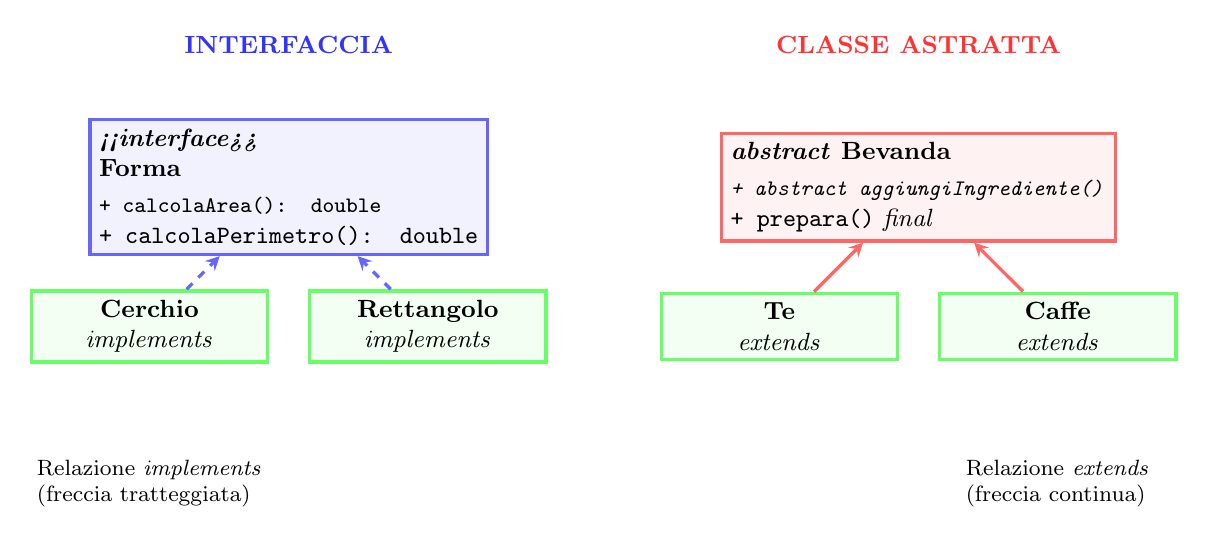
\begin{tikzpicture}[
    node distance=2.5cm,
    interface/.style={
        rectangle,
        draw=blue!60,
        fill=blue!5,
        very thick,
        minimum width=4cm,
        minimum height=0.8cm,
        align=left,
        font=\small
    },
    abstract/.style={
        rectangle,
        draw=red!60,
        fill=red!5,
        very thick,
        minimum width=4cm,
        minimum height=0.8cm,
        align=left,
        font=\small
    },
    concrete/.style={
        rectangle,
        draw=green!60,
        fill=green!5,
        very thick,
        minimum width=3cm,
        minimum height=0.8cm,
        align=center,
        font=\small
    },
    arrow/.style={
        ->,
        >=stealth,
        very thick
    }
]

% Parte sinistra - Interfaccia
\node[interface] (iforma) at (0,0) {
    \textbf{\textit{<<interface>>}}\\
    \textbf{Forma}\\[2pt]
    \footnotesize
    \texttt{+ calcolaArea(): double}\\
    \texttt{+ calcolaPerimetro(): double}
};

\node[concrete, below left of=iforma, node distance=2.5cm] (icerchio) {
    \textbf{Cerchio}\\
    \textit{implements}
};

\node[concrete, below right of=iforma, node distance=2.5cm] (irett) {
    \textbf{Rettangolo}\\
    \textit{implements}
};

\draw[arrow, blue!60, dashed] (icerchio) -- (iforma);
\draw[arrow, blue!60, dashed] (irett) -- (iforma);

% Parte destra - Classe astratta
\node[abstract, right of=iforma, node distance=8cm] (abevanda) {
    \textbf{\textit{abstract} Bevanda}\\[2pt]
    \footnotesize
    \texttt{\textit{+ abstract aggiungiIngrediente()}}\\
    \texttt{+ prepara()} \textit{final}
};

\node[concrete, below left of=abevanda, node distance=2.5cm] (te) {
    \textbf{Te}\\
    \textit{extends}
};

\node[concrete, below right of=abevanda, node distance=2.5cm] (caffe) {
    \textbf{Caffe}\\
    \textit{extends}
};

\draw[arrow, red!60] (te) -- (abevanda);
\draw[arrow, red!60] (caffe) -- (abevanda);

% Etichette
\node[above of=iforma, node distance=1.8cm, font=\small\bfseries, blue!80] {INTERFACCIA};
\node[above of=abevanda, node distance=1.8cm, font=\small\bfseries, red!80] {CLASSE ASTRATTA};

% Legenda
\node[below of=icerchio, node distance=2cm, font=\footnotesize, align=left] {
    Relazione \textit{implements}\\
    (freccia tratteggiata)
};

\node[below of=caffe, node distance=2cm, font=\footnotesize, align=left] {
    Relazione \textit{extends}\\
    (freccia continua)
};

\end{tikzpicture}
\caption{Confronto visuale tra interfaccia (Forma) e classe astratta (Bevanda). Le interfacce definiscono solo contratti, mentre le classi astratte possono contenere implementazioni}
\label{fig:interfacce_vs_classi_astratte}
\end{figure}

\subsection{Quando usare interfacce}

Usa le interfacce quando:
\begin{itemize}
    \item Vuoi definire un contratto (un insieme di metodi) senza vincolare l'implementazione
    \item Classi non correlate gerarchicamente devono avere comportamenti comuni
    \item Serve supporto per ereditarietà multipla di comportamento (una classe può implementare più interfacce)
    \item Vuoi definire tipi per il polimorfismo senza imporre una relazione "is-a" stretta
    \item Non hai bisogno di condividere codice o stato tra le classi implementanti
\end{itemize}

\textbf{Esempi dalla libreria Java:} \texttt{Serializable}, \texttt{Comparable}, \texttt{Runnable}, \texttt{Cloneable} sono interfacce perché definiscono capacità/comportamenti che classi di tipo completamente diverso possono implementare, senza alcuna relazione gerarchica tra loro.

\subsection{Quando usare classi astratte}

Usa le classi astratte quando:
\begin{itemize}
    \item Vuoi condividere codice (metodi concreti) tra classi strettamente correlate
    \item Devi mantenere stato comune (variabili di istanza/attributi) tra le sottoclassi
    \item Vuoi fornire un'implementazione di default per alcuni metodi, lasciando altri astratti
    \item Le classi derivate hanno una relazione "is-a" forte con la classe base (es. Auto IS-A Veicolo)
    \item Hai bisogno di costruttori per inizializzare lo stato comune
    \item Vuoi usare modificatori di accesso diversi da \texttt{public} per i metodi
\end{itemize}

\textbf{Esempi dalla libreria Java:} \texttt{InputStream}, \texttt{OutputStream}, \texttt{AbstractList} sono classi astratte perché definiscono funzionalità comuni a tutte le sottoclassi con implementazioni parzialmente condivise e stato comune.

\begin{nota}
Regola pratica: preferisci le interfacce alle classi astratte per massima flessibilità. Usa classi astratte quando hai davvero bisogno di condividere implementazione o stato.
\end{nota}

\section{Polimorfismo con interfacce e classi astratte}

Il vero potere di interfacce e classi astratte emerge con il polimorfismo: la possibilità di trattare oggetti di classi diverse attraverso un tipo comune.

\subsection{Esempio 5: Polimorfismo con array}

\begin{lstlisting}
public interface Suonabile {
    // Metodi astratti dell'interfaccia
    void suona();
    void accordatura();
}

public class Chitarra implements Suonabile {
    // Implementazione del metodo chitarra.suona()
    @Override
    public void suona() {
        System.out.println("Suonando la chitarra: strum strum");
    }

    // Implementazione del metodo chitarra.accordatura()
    @Override
    public void accordatura() {
        System.out.println("Accordando le corde della chitarra");
    }
}

public class Piano implements Suonabile {
    // Implementazione del metodo piano.suona()
    @Override
    public void suona() {
        System.out.println("Suonando il piano: ding ding");
    }

    // Implementazione del metodo piano.accordatura()
    @Override
    public void accordatura() {
        System.out.println("Accordando le corde del piano");
    }
}

public class Batteria implements Suonabile {
    // Implementazione del metodo batteria.suona()
    @Override
    public void suona() {
        System.out.println("Suonando la batteria: boom boom");
    }

    // Implementazione del metodo batteria.accordatura()
    @Override
    public void accordatura() {
        System.out.println("Regolando la tensione dei tamburi");
    }
}

// Uso del polimorfismo
public class Concerto {
    public static void main(String[] args) {
        // Array di tipo interfaccia con oggetti di classi diverse
        Suonabile[] strumenti = {
            new Chitarra(),
            new Piano(),
            new Batteria()
        };

        // Itera e suona tutti gli strumenti
        System.out.println("=== CONCERTO ===");
        for (Suonabile s : strumenti) {
            s.accordatura();  // Chiama il metodo s.accordatura()
            s.suona();        // Chiama il metodo s.suona()
            System.out.println();
        }
    }
}
\end{lstlisting}

Questo esempio dimostra il \textbf{polimorfismo in azione} attraverso le interfacce, uno dei concetti più potenti della programmazione orientata agli oggetti. L'interfaccia \texttt{Suonabile} definisce due metodi comuni a tutti gli strumenti musicali: il metodo \texttt{oggetto.suona()} e il metodo \texttt{oggetto.accordatura()}. Le tre classi concrete (\texttt{Chitarra}, \texttt{Piano}, \texttt{Batteria}) implementano questa interfaccia, ciascuna con il proprio comportamento specifico: la chitarra fa "strum strum", il piano "ding ding", la batteria "boom boom". L'aspetto chiave è nella classe \texttt{Concerto}: possiamo creare un array di tipo \texttt{Suonabile[]} che contiene oggetti di classi completamente diverse. Quando iteriamo sull'array e chiamiamo il metodo \texttt{s.suona()}, Java determina automaticamente a runtime quale implementazione chiamare in base al tipo reale dell'oggetto (questo si chiama \textbf{binding dinamico} o \textbf{late binding}). Lo stesso vale per il metodo \texttt{s.accordatura()}. Questo permette di scrivere codice generico che funziona con qualsiasi strumento musicale, presente o futuro, purché implementi l'interfaccia \texttt{Suonabile}. Se domani vogliamo aggiungere un violino, basta creare una nuova classe che implementa l'interfaccia, e funzionerà automaticamente con tutto il codice esistente.

\begin{errore}
Non confondere il tipo dichiarato con il tipo reale dell'oggetto. Se hai \texttt{Forma f = new Cerchio()}, puoi chiamare solo i metodi dell'interfaccia \texttt{Forma} sulla variabile \texttt{f}, anche se l'oggetto è effettivamente un \texttt{Cerchio}. Per accedere a metodi specifici della classe \texttt{Cerchio} serve il casting esplicito: \texttt{((Cerchio)f).metodoSpecifico()}.
\end{errore}

\section{Esempio pratico completo: Sistema geometrico}

\begin{lstlisting}
// Interfaccia base
public interface Forma {
    // Metodi astratti dell'interfaccia
    double area();
    double perimetro();
}

// Classe astratta che implementa parzialmente l'interfaccia
public abstract class FormaConColore implements Forma {
    // Attributo di istanza condiviso
    protected String colore;

    // Costruttore della classe astratta
    public FormaConColore(String colore) {
        this.colore = colore;
    }

    // Metodo concreto forma.stampaInfo()
    // Utilizza l'attributo colore e i metodi astratti area() e perimetro()
    public void stampaInfo() {
        System.out.println("Forma di colore " + colore);
        System.out.println("Area: " + area());
        System.out.println("Perimetro: " + perimetro());
    }

    // I metodi area() e perimetro() rimangono astratti
    // Le sottoclassi devono implementarli
}

// Implementazioni concrete
public class Quadrato extends FormaConColore {
    // Attributo specifico del quadrato
    private double lato;

    // Costruttore: chiama super() per inizializzare l'attributo colore
    public Quadrato(String colore, double lato) {
        super(colore);
        this.lato = lato;
    }

    // Implementazione del metodo quadrato.area()
    @Override
    public double area() {
        return lato * lato;
    }

    // Implementazione del metodo quadrato.perimetro()
    @Override
    public double perimetro() {
        return 4 * lato;
    }
}

public class Triangolo extends FormaConColore {
    // Attributi specifici del triangolo
    private double base;
    private double altezza;
    private double lato1, lato2, lato3;

    // Costruttore: chiama super() per inizializzare l'attributo colore
    public Triangolo(String colore, double base, double altezza,
                     double lato1, double lato2, double lato3) {
        super(colore);
        this.base = base;
        this.altezza = altezza;
        this.lato1 = lato1;
        this.lato2 = lato2;
        this.lato3 = lato3;
    }

    // Implementazione del metodo triangolo.area()
    @Override
    public double area() {
        return (base * altezza) / 2;
    }

    // Implementazione del metodo triangolo.perimetro()
    @Override
    public double perimetro() {
        return lato1 + lato2 + lato3;
    }
}

// Test del polimorfismo
public class TestGeometria {
    public static void main(String[] args) {
        // Array di tipo FormaConColore con oggetti di classi diverse
        FormaConColore[] forme = {
            new Quadrato("Rosso", 5),
            new Triangolo("Blu", 4, 3, 3, 4, 5)
        };

        // Itera e stampa informazioni di tutte le forme
        for (FormaConColore f : forme) {
            f.stampaInfo();  // Chiama il metodo f.stampaInfo()
            System.out.println("---");
        }
    }
}
\end{lstlisting}

Questo esempio completo combina \textbf{interfacce e classi astratte}, dimostrando come possano lavorare insieme in un design ben strutturato. L'interfaccia \texttt{Forma} definisce il contratto base (i metodi \texttt{oggetto.area()} e \texttt{oggetto.perimetro()}), ma non può contenere variabili di istanza. La classe astratta \texttt{FormaConColore} implementa parzialmente l'interfaccia: aggiunge la variabile di istanza \texttt{colore} e il metodo concreto \texttt{oggetto.stampaInfo()}, ma lascia astratti i metodi \texttt{area()} e \texttt{perimetro()} perché il calcolo dipende dalla forma specifica. Il metodo \texttt{stampaInfo()} utilizza internamente l'attributo \texttt{colore} e i metodi \texttt{area()} e \texttt{perimetro()} per stampare le informazioni. Le classi concrete \texttt{Quadrato} e \texttt{Triangolo} estendono \texttt{FormaConColore} e forniscono le implementazioni finali dei metodi astratti utilizzando i propri attributi specifici (come \texttt{lato} per il quadrato e \texttt{base}, \texttt{altezza} per il triangolo). Questo approccio a tre livelli è molto comune nelle applicazioni reali: l'interfaccia definisce il comportamento pubblico, la classe astratta fornisce funzionalità comuni e mantiene stato condiviso, le classi concrete implementano i dettagli specifici. Nota come nel test possiamo usare polimorfismo: entrambe le forme vengono trattate attraverso il tipo \texttt{FormaConColore}, ma ognuna esegue i propri calcoli specifici quando si chiamano i metodi \texttt{f.area()} e \texttt{f.perimetro()}.

\section*{Riepilogo}

In questo capitolo abbiamo imparato:

\begin{itemize}
    \item L'\textbf{astrazione} è un principio fondamentale della OOP che definisce "cosa fa" un oggetto senza specificare "come lo fa"
    \item Le \textbf{interfacce} definiscono contratti (insiemi di metodi astratti) che le classi devono implementare completamente
    \item Le \textbf{classi astratte} possono contenere sia metodi astratti che metodi concreti, e possono mantenere stato (attributi)
    \item Una classe può implementare \textbf{più interfacce} contemporaneamente ma può estendere \textbf{una sola classe} (astratta o concreta)
    \item Interfacce e classi astratte sono strumenti fondamentali per realizzare il \textbf{polimorfismo} in Java
    \item Regola pratica: usa interfacce per definire comportamenti/capacità comuni, usa classi astratte per condividere implementazione e stato tra classi correlate
    \item L'annotazione \textbf{\texttt{@Override}} è fondamentale quando si implementano metodi di interfacce o si sovrascrivono metodi astratti
\end{itemize}

\begin{nota}
\textbf{Best Practices:}
\begin{itemize}
    \item Preferisci interfacce alle classi astratte per massima flessibilità e riusabilità
    \item Usa nomi descrittivi: le interfacce spesso terminano con "-able" per indicare capacità (\texttt{Comparable}, \texttt{Runnable}, \texttt{Serializable})
    \item Mantieni le interfacce piccole e focalizzate su un unico scopo (Interface Segregation Principle - ISP)
    \item Documenta chiaramente il contratto definito dall'interfaccia e le responsabilità dei metodi
    \item Usa classi astratte quando devi condividere codice comune (metodi concreti) e stato (attributi) tra classi strettamente correlate
    \item Usa l'annotazione \texttt{@Override} quando implementi metodi di interfacce o sovrascrivi metodi astratti
\end{itemize}
\end{nota}

\begin{errore}
\textbf{Errori comuni da evitare:}
\begin{itemize}
    \item Tentare di istanziare direttamente interfacce o classi astratte con l'operatore \texttt{new} (genera errore di compilazione)
    \item Dimenticare di implementare tutti i metodi astratti dell'interfaccia nelle classi concrete
    \item Non usare l'annotazione \texttt{@Override} quando si implementano metodi di interfacce o si sovrascrivono metodi astratti (l'annotazione aiuta a catturare errori di battitura)
    \item Confondere la relazione di ereditarietà (\texttt{extends}) con la relazione di implementazione (\texttt{implements})
    \item Usare classi astratte quando basterebbe un'interfaccia (perdita di flessibilità)
    \item Creare interfacce troppo grandi con molti metodi non correlati (viola il principio ISP)
\end{itemize}
\end{errore}

\section*{Riferimenti per approfondimenti}

\begin{itemize}
    \item Oracle Java Tutorial - Interfaces: \url{https://docs.oracle.com/javase/tutorial/java/IandI/createinterface.html}
    \item Oracle Java Tutorial - Abstract Classes: \url{https://docs.oracle.com/javase/tutorial/java/IandI/abstract.html}
    \item Effective Java (Joshua Bloch) - Item 20: Prefer interfaces to abstract classes
    \item Design Patterns (Gang of Four) - Template Method Pattern
\end{itemize}
